\documentclass[../Text/00main.tex]{subfiles}
\graphicspath{{../}}

\begin{document}


\section{The Centroid Moment Tensor}\label{sec:CMTexplanation}


\begin{figure}
    \centering
    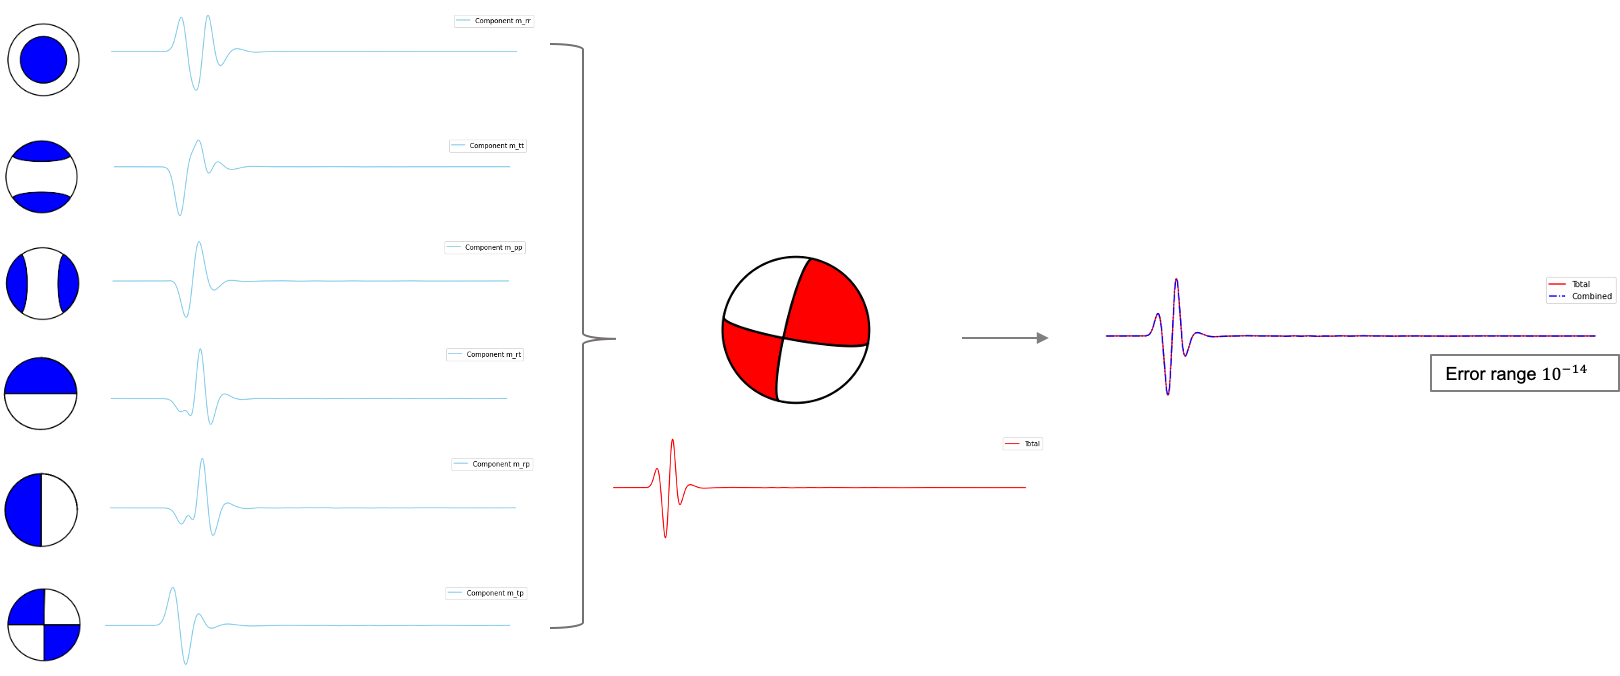
\includegraphics[width=.85\textwidth]{images_methods/cmtcombi_informationfigure.png}
    \caption{The six CMT components represented by their respective focal mechanisms. They can be summed to create the total moment tensor. When compared to the result of a simulation run with a total moment tensor solution, the error is below the floating-point range.}
    \label{fig:cmtseparatecombine}
\end{figure}

\begin{figure}
    \centering
    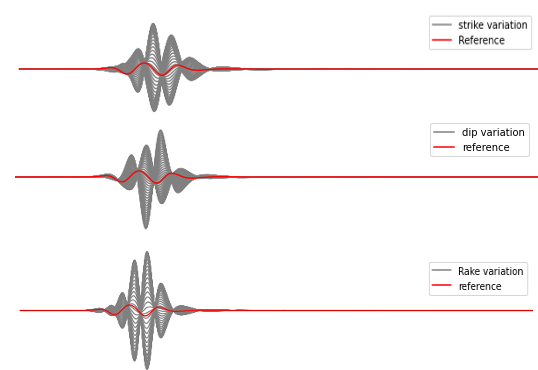
\includegraphics[width=.75\textwidth]{images_methods/expl_sdrvar_prettyfigure.png}
    \caption{Strike, dip and rake variation in both directions (+/- 45 $\degree$) and their influence on the total signal.}
    \label{fig:cmtprettyfigure}
\end{figure}

A moment tensor is a representation of the non-elastic deformation at the source location that takes place at the event. It is a second-order tensor $M_{ij}$ with on its diagonal axis the isotropic components of the source, and on the off-diagonal elements the deviatoric components, representing the nine generalised couples of the source \cite{richards1980quantitative}. The moment tensor can represent both an extended source or a point source approximation.

The Centroid Moment Tensor (CMT) approximation is a commonly used method to represent the seismic source of an earthquake. It is a comprehensive and computationally inexpensive way to represent the mechanism behind an event. The symmetry of the deviatoric components reduces the number of moment tensor components to 6, represented with their compressional patterns on the focal sphere in Figure \ref{fig:cmtseparatecombine}. Related to the more geological dimensions of a seismic event, the six moment tensor components are multiplied by the seismic moment $M_{0}$ derived from the strike $\phi$, dip $\delta$ and rake $\lambda$ of the fault as such:

\begin{equation}
\begin{array}{l}M_{\mathrm{11}}=-M_{0}\left(\sin \delta \cos \lambda \sin 2 \phi+\sin 2 \delta \sin \lambda \sin ^{2} \phi\right) ,\\ M_{\mathrm{12}}=M_{0}(\sin \delta \cos \lambda \cos 2 \phi+0.5 \sin 2 \delta \sin \lambda \sin 2 \phi) ,\\ M_{\mathrm{13}}=-M_{0}(\cos \delta \cos \lambda \cos \phi+\cos 2 \delta \sin \lambda \sin \phi) ,\\ M_{\mathrm{22}}=M_{0}\left(\sin \delta \cos \lambda \sin 2 \phi-\sin 2 \delta \sin \lambda \cos ^{2} \phi\right) ,\\ M_{\mathrm{23}}=-M_{0}(\cos \delta \cos \lambda \sin \phi-\cos 2 \delta \sin \lambda \cos \phi) ,\\ M_{\mathrm{33}}=M_{\mathrm{o}} \sin 2 \delta \sin \lambda.
\end{array}
\end{equation}

The relation between moment magnitude $M_w$ and seismic moment $M_0$ (\cite{hanks1979moment}) in N m is given by:

\begin{equation}
    M_w = \frac{2}{3}(log_{10} M_0 - 9.1),
\end{equation} 

with earthquake magnitude and rupture area are proportional to each other by $$M_0 = \mu AD$$. Realistically, a moderate to large event has a large rupture area and can not be adequately represented by a point source. In the pilot demonstrator for ChEESE, the first post-event step of an urgent seismic simulation is determining the CMT solution for the event source. The next step of the urgent seismic simulation protocol would be a more realistic source model with a finite rupture such as \cite{graves_kinematic_2016}. However, the amount of parameters to be chosen and the high computational cost of this more realistic rupture model make this type of source modelling prohibitive to use when even the CMT solution is uncertain. The rapid post-event source estimates must therefore first provide a CMT solution. The CMT is a moment tensor that is located at the "centre of mass" of a seismic event. This is usually located roughly at the middle of the fault rupture and at half the source time duration \cite{dziewonski_determination_1981}. For some earthquakes, post-event inversion for the moment tensor is done by institutions such as the Global Centroid Moment Tensor catalogue (GCMT, \cite{ekstromdziewo}, \cite{dziewonski_determination_1981}), by constraining the isotropic components of the moment tensor to zero, implying zero volumetric change. Body waves, mantle waves and surface waves are then used for inversion of the deviatoric components. In case of the GCMT, this is done up to a period of 40s for the six moment tensor components, the location in latitude, longitude, and the depth. In the case of a "fixed" inversion, the location is set a-priori, this is done for earthquakes shallower than 12 km. The GCMT catalogue provides a standard error for the six moment tensor components. Adding to the moment tensor component uncertainty, location of the CMT is not constrained well. Latitude, longitude, depth and moment tensor components vary with the wavelengths and wave-types used during the inversion, see e.g. \cite{valentine_assessing_2012}. Especially depth is poorly constrained, but may have major implications on ground motion. The amount of coverage of an event by seismic stations grossly influences the quality of the source inversion. Not all events with a damage potential are captured by these catalogues, prompting the first workflow step of ChEESE as near-realtime source inversion.

\hl{To do: insert image of strike-dip and rake}

\section{The spectral element method}

The spectral element method (SEM) is used as the numerical method to model the propagation of the seismic wavefield for our reference earthquake scenarios. SEM is a class of Finite Element Methods, benefiting from the implicit free surface property and it proves to be very well suited for discretisations of domains with complex topography \cite{fichtner_deep_2013}. Spatial discretisation of hexahedral elements and a Finite-Difference time-stepping method approximate the solution of the wave-equation at each point. The discretised wave-equation is represented by the following global equation

\begin{equation}
    \mathbf{M}\partial^2_t\mathbf{u}(t) +
    \mathbf{Ku}(t) =
    \mathbf{f}(t),
    \label{eq:mutkutglobal}
\end{equation}

with $\mathbf{u}$ the unknown wavefield solved at each point, $\mathbf{K}$ the stiffness matrix, $\mathbf{M}$ the mass matrix and $\mathbf{f}$ the volumetric force vector. It makes use of fourth-order Lagrange polynomials as interpolation functions, with Gauss-Lobatto-Legendre (GLL) collocation points. GLL points are the roots  of the first derivative of the Legendre polynomials and allow for an optimal spatial point distribution \cite{igel_spectral-element_2016}. Usage of these GLL points as quadrature points makes the mass matrix $\mathbf{M}$ diagonal and thus trivially invertible. Other type of meshes than hexahedral meshes can be used, but then this favourable diagonal property is lost. The time-stepping scheme allows for relatively straightforward paralellisation of simulations. The wavefield solution for the next time step $t + dt$ is computed as

\begin{equation}
\mathbf{u}_{g}(t+d t)= dt^{2}\left[\mathbf{M}_{g}^{-1}\left(\mathbf{f}_{g}(t)
-\mathbf{K}_{g} \mathbf{u}_{g}(t)\right)\right] 
+ 2 \mathbf{u}_{g}(t)-\mathbf{u}_{g}(t-d t) ,
\end{equation} 

where the subscript $g$ denotes that the solution is global. This time discretisation renders the method particularly suitable for large-scale wave propagation simulations that make use of HPC resources. The method was adapted for 3D wave propagation by \cite{komatitsch1999introduction} and is now one of the more widely used methods for deterministic seismic simulations. \cite{igel_spectral-element_2016} offers a more extensive explanation of the spectral element method. 

\section{Gound motion parameters}

\hl{To do: create a comprehensive overview figure for ground motion parameters}

It is key to express the abundance of information that can be obtained from a seismogram as meaningful parameters. Ground motion parameters (GMP) or inensity measures (IM), are measures of the ground motions derived from these seismic records, or from civil surveys such as the USGS "Did You Feel It" index (DYFI, \cite{atkinson2007did}). The commonly analysed ground motion parameters derived from records can be sub-divided into three main categories: duration-based, peak-based and spectral parameters. In this section we explain the definition of the parameters used to compare to recorded data and map out the earthquake response in this study. 

\subsection{Peak Ground Acceleration (PGA)}

The Peak Ground Acceleration (PGA) corresponds to the highest amplitude of the acceleration time series of the earthquake signal at a given station. It is a much-used parameter in seismic hazard assessment and a map of the PGA is often published after a significant event.

\begin{equation}
    PGA = max(\mid a(t) \mid)
\end{equation}

The PGA is an indicator of the severity of the ground accelerations during an event, and is used for structural engineering purposes. However, the duration or spectrum of the event is not captured by this parameter. Thus, a high PGA does not always represent the same amount of damage. The PGA is mostly used for relatively short-period waves and in earthquake engineering for shorter buildings (back this up with reference!). It directly represents the horizontal force that a building is subjected to during an event. 

\subsection{Peak Ground Velocity (PGV)}

The Peak Ground Velocity (PGV) represents the highest amplitude of the velocity time series of the earthquake signal at a given station. 

\begin{equation}
    PGV = max(\mid v(t) \mid)
\end{equation}

The PGV is also used as damage indicator, and is less sensitive to higher-frequency content than the PGA (\cite{kramer:1996}). The PGV is used for earthquake building engineering for the modelling of taller buildings (how many stories?) and is the primary measure in more severe earthquakes (reference?).  

\subsection{Arias Intensity}

The Arias intensity, introduced by \cite{arias1970measure}, is a measure of the intensity of a signal and its impact for a uniform population of structures. The intensity is an of the integral over the acceleration time series $a$ squared for the duration of the signal $T_d$, multiplied with  $\frac{\pi}{2}$:

\begin{equation}
    I_A = \frac{\pi}{2g} \int_0^{T_d} a(t)^2 dt
\end{equation}

with $g$ the acceleration of gravity. The measure captures the amplitude, duration and frequency content of the signal and is a common proxy used in earthquake engineering \cite{howard2008probabilistic}. It captures well the short-period structural response \cite{travasarou2003empirical}. 

\subsection{Energy integral}

The Energy integral is similar to the Arias intensity, and gives the total energy over the duration of the velocity time series. 

\begin{equation}
    I_E = \int_0^{T_d} v(t)^2 dt
\end{equation}

\subsection{Spectral Response}

The spectral response is a popular parameter for earthquake engineering purposes. It represents the peak spectral acceleration for each frequency-band of the signal.  The spectrum represents a series of oscillators that oscillate at their respective natural frequencies. The spectral acceleration is often used for modelling the force a building is subjected to during an earthquake. We plot a 5\% damped pseudo-spectral acceleration spectra (Ssa) against natural periods $T_d$. 


% \section{Increasing realistic complexity: topography and ocean}

% It has been demonstrated by (\hl{papers met ook die van Marta}) that including the topography in the simulation domain can have significant effects on duration, ... (\hl{ETC, beetje uitleg!!}) of the earthquake signal. 

% To this end, the influence of topography is taken into account ...

% As discussed in Section \ref{CH1sec:Tectonics}, 

\section{Towards a realistic domain: topography and ocean}


\subsection{Topography effects}

Topography has been proven to influence duration, spectral content, amplification and de-amplification of seismic waves, e.g. \cite{veeraraghavan_simulation_2020}, \cite{pienkowska2020high}. This may have significant effects on the intensity measures that are studied in the context of this thesis. \cite{veeraraghavan_simulation_2020} shows that amplification takes place at ridges and de-amplification at the foot of steep topographical features. Primarily the sub-surface exhibits steep topography in the Marmara region considered here, as discussed in section \ref{CH1sec:Tectonics}. The spectral element method is well suited for domains with complex surface topography. 



\subsection{Ocean coupling}

When modeling frequencies < 10 seconds, crustal features, effects of a deep water layer in the domain as well as an undulating bathymetry, start to become increasingly important for realistic forward modelling. PwP waves, travelling up to the water surface and bouncing back into the crust, as well as frequencies travelling in the SOFAR channel have a frequency content of a few seconds \cite{fernando2020oceanic}. The oceanic layer is often accounted for as an oceanic load. This entails accounting for the weight of the ocean and setting the shear modulus to zero, without actually having to implement the ocean in the mesh. This formulation however only proves valid if the water column height is only a fraction of the dominant wavelength of the simulation \cite{komatitsch2002spectral}. If the water column becomes sufficiently deep, or the frequency increases, the simulation should be done in a solid-fluid coupled fashion. The boundary condition at the surface now changes from a Neumann to a Dirichlet condition. In addition to the deformed mesh due to undulating bathymetry, a finer discretization in space and time have to account for the lower velocities in the water layer in order to adhere to the Nyquist criterion. 

\hl{to be continued}


% \cite{afanasiev2019modular}
% \cite{qu2020fluid}

% \cite{fernando2020oceanic}

% cite
% Seismic forward modeling in fluid–solid media based on equivalent staggered grid scheme

% Forward modeling of ocean-bottom cable data and wave-mode separation in fluid–solid elastic media with irregular seabed
% . \cite{petukhin2010study}, \ 

% Finite difference seismic forward modeling method for fluid–solid coupled media with irregular seabed interface 







\end{document}